\documentclass{article}
\usepackage{graphicx}
\usepackage{fitbox}
\usepackage{subfig}
\begin{document}

The use of fitbox with a subfigure.  Note that the optional argument
for the command counts the lines for the subcaptions.  

\SetFitboxLayout[1]{2}{3}




\begin{figure}
  \centering
  \subfloat[First
  Napoleon]{\fitbox*{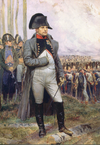
\includegraphics{napoleon}}}~
  \subfloat[Second
  Napoleon]{\fitbox*{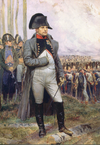
\includegraphics{napoleon}}}~
  \subfloat[Third
  Napoleon]{\fitbox*{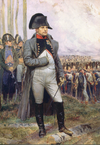
\includegraphics{napoleon}}}\\
  \subfloat[Fourth
  Napoleon]{\fitbox*{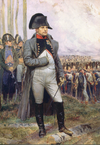
\includegraphics{napoleon}}}~
  \subfloat[Fifth
  Napoleon]{\fitbox*{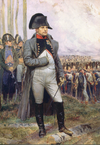
\includegraphics{napoleon}}}~
  \subfloat[Sixth
  Napoleon]{\fitbox*{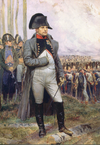
\includegraphics{napoleon}}}
  \caption{Six Napoleons}
  \label{fig:napoleons}
\end{figure}

\SetFitboxLayout{3}{2}

\begin{figure}
  \centering
  \subfloat{\fitbox*{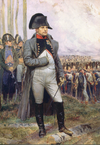
\includegraphics{napoleon}}}~
  \subfloat{\fitbox*{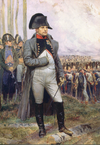
\includegraphics{napoleon}}}~
  \subfloat{\fitbox*{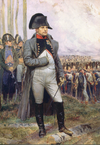
\includegraphics{napoleon}}}\\
  \subfloat{\fitbox*{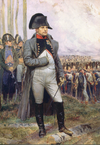
\includegraphics{napoleon}}}~
  \subfloat{\fitbox*{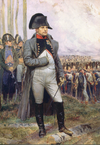
\includegraphics{napoleon}}}~
  \subfloat{\fitbox*{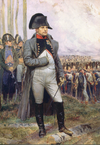
\includegraphics{napoleon}}}
  \caption{Six Napoleons, no subcaptions}
  \label{fig:napoleons1}
\end{figure}

\SetFitboxLayout[1]{3}{2}




\begin{figure}
  \centering
  \subfloat[First
  Napoleon]{\fitbox*{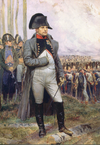
\includegraphics{napoleon}}}~
  \subfloat[Second
  Napoleon]{\fitbox*{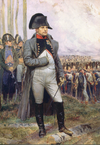
\includegraphics{napoleon}}}\\
  \subfloat[Third
  Napoleon]{\fitbox*{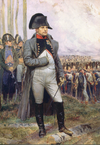
\includegraphics{napoleon}}}~
  \subfloat[Fourth
  Napoleon]{\fitbox*{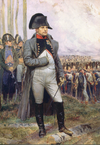
\includegraphics{napoleon}}}\\
  \subfloat[Fifth
  Napoleon]{\fitbox*{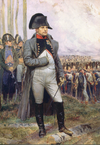
\includegraphics{napoleon}}}~
  \subfloat[Sixth
  Napoleon]{\fitbox*{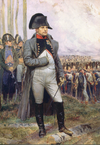
\includegraphics{napoleon}}}
  \caption{Six Napoleons, another arrangement}
  \label{fig:napoleons3}
\end{figure}


\end{document}
